\chapter{Introduction}
\label{chap:intro}

The use of high performance computers for  research in the Faculty of Engineering  and Scientific has increase, because of increase in research tasks, such as testing new operating systems. As researchers demand large data storage and robust computer architectures, these computer systems and their properties  also need to be expanded to accommodate this large tasks. As we expand the systems access and usage  becomes more complicated to manage. Therefore we are faced with the issue of system management, system accessibility, and storage. These issues for example, are the inability to provide proper record of each computer system and their usage, the inability to provide flexible users access to the computers, and also the problem of monitoring the number of computers that are reserved by users. As a result of these challenges it is highly necessary to develop software that solves these problems for Faculty of Engineering and Science. 


Clowder is a system designed to provide Preboot Execution Environment (PXE) for testing new operating systems through a Network File System (NFS) sever on the high performance computers. Previous work has been started by researchers in Engineering department to complete these system for several years, but yet there was more improvement yet to be made in order to complete it, as it lacks some necessary modern functionality and features, such as database system, interactive user interface  and restrictions.  As an example, it takes extra effort and manual command line statements to access  a computer in the cluster during research. Another reason for improvement is to provide flexible and dynamic user interface rather than current one (SSH). Therefore the current state of Clowder is not flexible and convenient enough. So the main goal of this project is to develop software that addresses the issue of user accessibility, system management and automatic control protocol. Addressing all these issues will improve the performance of Clowder in speed , access and robustness, and therefore making it a completed software tool. 
	
	
We have accomplished this goal by using a design approach that provides a web interface, a databases system and automatic command protocols. The database system is designed to store and keep record of the computer systems and user activities. The web interface enable users to remotely log on to several machine from different locations simultaneously via a web page, and also provide user with the system inventory and other user activities. This  software provide the ability to adding new computer system to the cluster, and to modify their properties individually. Also it provides the ability to make reservations: to allow users to reserve a computer for a certain period of time, and able to end reservations as well. A function to allow user search the inventory with some specifications according to their demands.   
	

As this software serves as a tool to manage the cluster of computers and user activities, it is important to know that  reservations made, computer details, network interface cards and disks are stored as data. So all the computer system installed in the cluster with their names, vendors, memory size, architecture, and micro architecture is stored in the database. And same is applicable to the disks, network interface cards and any other devices that could be part of the cluster. Data is represented as variables in their various data types in the database scheme.  All these information stored in the database tables servers as input  data for the program and out put for the inventory. This database scheme allows user to add or update new machines installed in the cluster, and therefore provide dynamic access to the machines. 

The web interface serves as a platform for users to interact with the system and overview other users activities via a  web page using designated URL. This interface has also replaced the SSH command line prompts which was the previous user interface for Clowder system. This choice provides flexible access and control to the system, by allowing users to log on to the system and make request of the inventory at any time through the web server.
The following figure show a genaral description of the Clowder system:

\begin{figure}[h]
  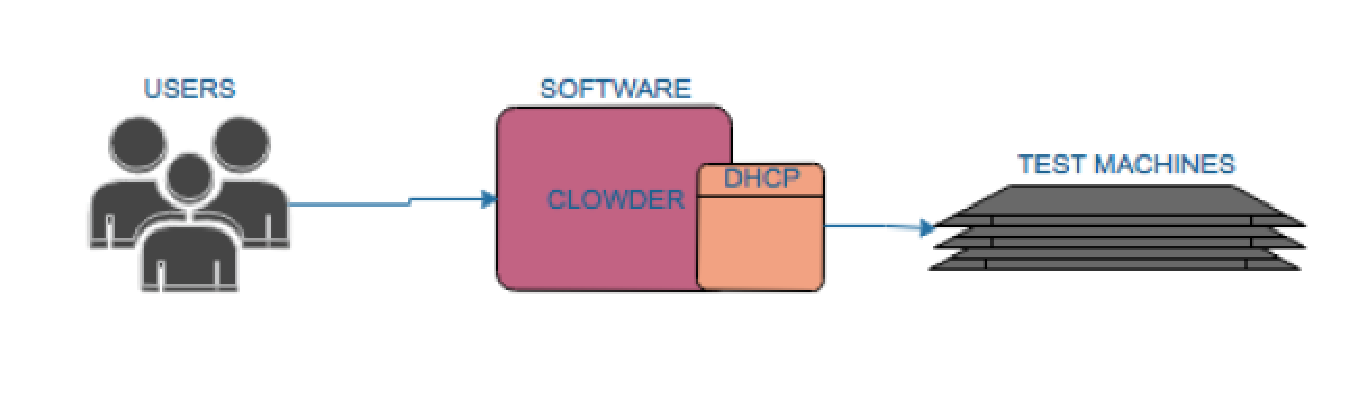
\includegraphics[width=\linewidth]{background.eps}
  \label{fig:Design of program}
  \caption{Design}
\end{figure}
\pagebreak

The above figure showcases the background concept of the Clowder as a full system. However, this concept has been made complete by designing a software that support the functionality required to have the a dynamic user interface and functional database. Following this chapter, we explain in more detail about the background of this system and other component that made up the design.
